\documentclass[a4paper,12pt]{report}

\usepackage[OT1]{fontenc}  %%%paket za kodiranje teksta T2 cirilica, T1 latinica%%%
\usepackage[english, croatian, serbian]{babel}
\usepackage[top= 27mm, bottom=27mm, left=25mm, right=25mm]{geometry}
\usepackage[utf8]{inputenc}
\usepackage{epstopdf}
\usepackage{graphicx}
\usepackage{enumerate}
\usepackage{amsmath,amsthm,amssymb}
\usepackage{hyperref}
\usepackage{multicol}
%\usepackage{multirow, multicol}
%\usepackage{array} 

\def\dj{d\kern-0.4em\char"16\kern-0.1em}
\def\Dj{\mbox{\raise0.3ex\hbox{-}\kern-0.4em D}}


\begin{document}

\begin{titlepage}

\newcommand{\HRule}{\rule{\linewidth}{0.5mm}} % Defines a new command for the horizontal lines, change thickness here

\center % Center everything on the page
 
%----------------------------------------------------------------------------------------
%	HEADING SECTIONS
%----------------------------------------------------------------------------------------

\textsc{\LARGE Matemati\v{c}ki fakultet}\\[1.5cm]

%\textsc{\LARGE Seminatski rad}\\[1.5cm] % Minor heading such as course title

%----------------------------------------------------------------------------------------
%	TITLE SECTION
%----------------------------------------------------------------------------------------
\vfill
\vfill

\vfill
\HRule \\[0.4cm]
{ \huge \bfseries Re\v{s}enja zadataka sa prijemnih ispita}\\[0.4cm] % Title of your document
\HRule \\[1.5cm]
 
%----------------------------------------------------------------------------------------
%	AUTHOR SECTION
%----------------------------------------------------------------------------------------
\vfill 



% If you don't want a supervisor, uncomment the two lines below and remove the section above
\emph{Autor:}\\
Ivana \textsc{Janki\'{c}}\\[3cm] % Your name

%----------------------------------------------------------------------------------------
%	DATE SECTION
%----------------------------------------------------------------------------------------

{\large \today}\\[3cm] % Date, change the \today to a set date if you want to be precise

%----------------------------------------------------------------------------------------
%	LOGO SECTION
%----------------------------------------------------------------------------------------

%\includegraphics[width=0.7\textwidth]{Logo.png}\\[1cm] % Include a department/university logo - this will require the graphicx package
 
%----------------------------------------------------------------------------------------

\end{titlepage}
%ne diram to je sadrzaj
\tableofcontents

\newpage

%\par sdfdsfdsgfdgfd\dj{}

%\begin{figure}[!h]
%\inlcudegraphics[width=0.7\textwidth]{slika.png}
%\caption{Naziv slike}
%Referenca na \cite{lit1}
%\end{figure}
%numeracija
%\begin{enumerate}[1]
%\item bla
%\end{enumerate}

%\begin{itemize}
%\item bla
%\end{itemize}

%\section{Naslov}
%dfjksfndlksjjfdklsjf

%\subsection{Podnaslov}

%\par \textbf{podebljan tekst} \emph{nagla\v{s}en tekst}

%\par \DJ{}ura\dj{} Brankovi\'c
%\newpage

%%%%%%%%%%%%%%%%%%%%%%%%%%%%%%%%%%%%%%%%%%%%%%%%%%%%%%%%%
%Odavde pocinjes sa textom
%
%
%\par sdfdsfdsgfdgfd\dj{}
%\newpage
%%%%%%%%%%%%%%%%%%%


%\section*{Uvod}
%\par Skripta je radjena od poslednjeg prijemnog ispita ka ranijima, p od 2016.
%\par DODATI JOS STVAARI :D

%\begin{figure}[!h]
%\begin{center}
%\includegraphics[width=0.7\textwidth]{slika1.jpg}
%\caption{NESTO}
%\end{center}
%\end{figure}
%\newpage                            

\chapter{Prijemni ispit iz 2016. godine}
%\addcontentsline{toc}{chapter}{Prijemni ispit iz 2016. godine}
\section{Zadaci}

\begin{enumerate}[1.]
\item Kada je 25\% kante prazno, ona sadr\v{z}i 25 litara vode vi\v{s}e nego kada je 25\% kante puno. Koliko litara vode sadr\v{z}i puna kanta?
%ovako se stavkjaju ponudjeni odg u istom redu
\begin{multicols}{5}
\begin{enumerate}[A)]
\item 25 \item 33 \item 50 \item 75 \item 90
\end{enumerate}
\end{multicols}

\item Dvocifreni zavr\v{s}etak prirodnog broja $a$ je 16. Ako broj $a$ nije deljiv sa 8, tada je cifra jedinica broja $3a/4$ jednaka:
\begin{multicols}{5}
\begin{enumerate}[A)]
\item 0 \item 2 \item 5 \item 7 \item 8
\end{enumerate}
\end{multicols}

\item Koliko ima prirodnih brojeva manjih od 1000000 koji su deljivi ta\v{c}no jednim od brojeva 11 i 13?
\begin{multicols}{5}
\begin{enumerate}[A)]
\item 6993 \item 153846 \item 160839 \item 167832 \item 993006
\end{enumerate}
\end{multicols}

\item Najveci koeficijent polinoma $(2x + 1)^{10} $ jednak je:
\begin{multicols}{5}
\begin{enumerate}[A)]
\item 120 \item 11520 \item 13440 \item 15360 \item 16480
\end{enumerate}
\end{multicols} 

\item Brojevi 2, $\sqrt{6} - \sqrt{2} $ i $4 - 2\sqrt{3}$ \v{c}ine prva tri \v{c}lana:
\begin{enumerate}[A)]
\item aritmeti\v{c}kog, ali ne i geometrijskog niza 
\item geometrijskog, ali ne i aritmeti\v{c}kog niza
\item i aritmeti\v{c}kog i geometrijskog niza
\item ni aritmeti\v{c}kog ni geometrijskog niza
\item niza sa op\v{s}tim \v{c}lanom $a_n = 4 - 2\sqrt{n} $
\end{enumerate}

\item Data je jedna\v{c}ina $\left(\frac{1 + ix}{1 - ix}\right)^2 = i $, gde je $x$ realna nepoznata. Broj re\v{s}enja ove jedna\v{c}ine u intervalu $(0,1/2)$ je:
\begin{multicols}{5}
\begin{enumerate}[A)]
\item 0 \item 1 \item 2 \item 4 \item $\infty$
\end{enumerate}
\end{multicols}

\item Ako su $x_1$ i $x_2$ re\v{s}enja jedan\v{c}ine $x^2 - x + 15 = 0$, tada je $x_1^3 + x_2^3 - 2x_1^2 - x_2^2 + x_1x_2 + 2x_1 + x_2 -15 $ jednako:
\begin{multicols}{5}
\begin{enumerate}[A)]
\item 1 \item 87 \item 31 \item 16 \item -14
\end{enumerate}
\end{multicols}

\item Ako su $a$ i $b$ realni brojevi takvi da polinom  $x^4 + ax^3 -ax +b $ daje ostatak $2x+4$  pri deljenju polinomom $x^2 + 2x+ 1$, tada je $ab$ jednako:
\begin{multicols}{5}
\begin{enumerate}[A)]
\item 1 \item 2 \item 3 \item 4 \item 5
\end{enumerate}
\end{multicols}

\item Date su funkcije  $ f_1(x) = \ln \frac{1 + \sin{x}}{1 - \sin{x}}$ , $ f_2(x) = \arcsin{x} \cdot \arctan{x} $, $ f_3(x) = \sin{x} + \cos{x} $ i $f_4(x) = \frac{\ln{x^2}}{\sqrt[3]{x}} $. Ako sa $p$ ozna\v{c}imo broj parnih, a sa $n$ broj neparnih me\dj{}u ovim funkcijama, ta\v{c}an je iskaz:
\begin{multicols}{3}
\begin{enumerate}[A)]
\item $p = 1$ i $n = 1$ \item $p = 2$ i $n = 2$ \item $p = 2$ i $n = 1$ \item $p = 1$ i $n = 2$ \item $p = 1$ i $n = 0$
\end{enumerate}
\end{multicols}



\item Za koje vrednosti realnog parametra $a$ jedna\v{c}ina $||x-3|-1|=a$ ima ta\v{c}no tri realna re\v{s}enja:
\begin{multicols}{5}
\begin{enumerate}[A)]
\item -1 \item 0 \item 1 \item 2 \item 3
\end{enumerate}
\end{multicols}


\item Funkcija $f$ je zadata sa $f(x) = \frac{ax +b}{cx+d} $, gde su $a,b,c$ i $d$ realni brojevi. Ako je $f(0) = 1$,  $f(1) = 0$ i  $f(2) = 3$, koliko je  $f(3)$?
\begin{multicols}{5}
\begin{enumerate}[A)]
\item -1 \item $\frac{3}{2}$ \item 5 \item 2 \item 3
\end{enumerate}
\end{multicols}


\item Broj re\v{s}enja sistema jedna\v{c}ina 
\par $(x^{2} - 1)(2x -3y + 4z) = 0$
\par $4x + 5y +8z = -2$
\par $3x + y + 6z = 44$
\par u skupu realnih brojeva je: 
\begin{multicols}{5}
\begin{enumerate}[A)]
\item 0 \item 1 \item 2 \item 3 \item $\infty$
\end{enumerate}
\end{multicols}

\item Ako za realne brojeve $x$  i $y$ va\v{z}i $7 \cdot 3^{x} - 5 \cdot 2^{y} = 23$ i $2 \cdot 3^{x} + 3 \cdot 2^{y} = 42$, onda je zbir $x + y$ jednak:
\begin{multicols}{5}
\begin{enumerate}[A)]
\item 7 \item 2 \item 3 \item 4 \item 5
\end{enumerate}
\end{multicols}


\item Proizvod svih re\v{s}enja jedna\v{c}ine $ \log_{36} x^{2} + \log_6 (x + 5) -1 = 0$ je :
\begin{multicols}{5}
\begin{enumerate}[A)]
\item -36 \item -6 \item 1 \item 12 \item 6
\end{enumerate}
\end{multicols}


\item Broj celobrojnih re\v{s}enja nejedna\v{c}ine $\sin{x} < \lvert \cos{x} \rvert $ u intervalu $[ 0,8] $ jednak je: 
\begin{multicols}{5}
\begin{enumerate}[A)]
\item 4 \item 5 \item 6 \item 7 \item 8
\end{enumerate}
\end{multicols}

\item Ta\v{c}ke $M,N$ i $P$ su sredi\v{s}ta tri me\d{j}usobno mimoilazne ivice kocke. Ako je du\v{z}ina ivice $4cm$, povr\v{s}ina trougla $MNP$ je:
\begin{multicols}{5}
\begin{enumerate}[A)]
\item $8\sqrt{2}cm^2$ \item $\sqrt{2}cm^2$ \item $8\sqrt{3}cm^2$ \item $8cm^2$ \item $6\sqrt{3}cm^2$
\end{enumerate}
\end{multicols}

\item Oko kru\v{z}nije opisan je \v{c}etvorougao $ABCD$ povr\v{s}ine $90cm^2$. Ako je zbir du\v{z}ina naspramnih stranica $AB$ i $CD$ jednak $15cm$, du\v{z}ina polupre\v{c}nika kru\v{z}nice je : 
\begin{multicols}{5}
\begin{enumerate}[A)]
\item $6cm$ \item $5\sqrt{2}cm$ \item $6\sqrt{3}cm$ \item $3\sqrt{3}cm$ \item $3cm$
\end{enumerate}
\end{multicols}

\item Date su dve koncentri\v{c}ne kru\v{z}nice i du\v{z} $AB$ koja je tetiva kru\v{z}nice ve\'{c}eg, a tangenta na kru\v{z}nicu manjeg polipre\v{c}nika. Ako je $AB = 6$, onda je povr\v{s}ina prstena izme\dj{}u datih kru\v{z}nica jednaka: 
\begin{multicols}{5}
\begin{enumerate}[A)]
\item $12\pi$  \item $9\pi$ \item $\pi$ \item 9 \item $6\pi$
\end{enumerate}
\end{multicols}

\item Povr\v{s}ina kvadrata \v{c}ije su dve stranice na pravima $2x + y - 3 = 0$, $2x +y -8 = 0$ je :
\begin{multicols}{5}
\begin{enumerate}[A)]
\item $2\sqrt{3}$  \item 5 \item 4 \item 6 \item $3\sqrt{2}$
\end{enumerate}
\end{multicols}

\item Du\v{z}ine stranica o\v{s}trouglog trougla su $a = 60$, $ b = 52$ i $c$, a veli\v{c}ine odgovaraju\'{c}ih uglova su $\alpha,\beta  $ i $\gamma $. Ako je $\sin{\alpha } = \frac{12}{13}$, onda je $\sin{\gamma }$ jednak:
\begin{multicols}{5}
\begin{enumerate}[A)]
\item $\frac{56}{65}$  \item $\frac{56}{63}$ \item $\frac{39}{65}$ \item $\frac{39}{63}$ \item $\frac{63}{65}$
\end{enumerate}
\end{multicols}

\end{enumerate}







%\begin{figure}[!h]
%\begin{center}
%\includegraphics[width=1.2\textwidth]{2016b.jpg}
%\caption{Druga strana}
%\end{center}
%\end{figure}

\newpage

\section{Re\v{s}enje}
\begin{enumerate}[1.]

\item 25\% kante je prazne je ekvivalnetno sa tim da je 75\% kante puno. Obele\v{z}imo sa $x$ zapreminu kante sa vodom. Prevedimo sada tekst zadatka u matemati\v{c}ki zapis:
\par Kada je 25\% kante prazno, ona sadr\v{z}i 25 litara vode vi\v{s}e nego kada je 25\% kante puno.
\par 75\% od $x$ umanjen sa 25 litara je isto sto i 25\% od $x$.
\par Matemati\v{c}ki : $ 0.75 \cdot x - 25 = 0.25 \cdot x$
\par Daljim re\v{s}avanjem ove jedna\v{c}ine dobijamo: $ 0.5 \cdot x = 25$. Ako obe strane pomo\v{z}imo sa brojem 2 dobijamo: $x = 50$, te je re\v{s}enja zadatka 50 litara. \textbf{Odgovor je pod C.}

\item Dvocifreni zavr\v{s}etak prirodnog broja $a$ je 16, matemati\v{c}ki zapisano $ a \equiv 16 \pmod{100}$. Znamo da 8 ne sme da deli $a$, dok po tekstu zadatka zaklju\v{c}ujemo da 4 mora da deli $a$. Uradimo zadatak pe\v{s}aka, ispi\v{s}imo sve dvocifrene i trocifrene brojeve kod kojih va\v{z}i gorenja relacija. Krenu\'{c}emo od 16 do 916.
\par 16 - ne mo\v{z}e jer je deljivo sa 8.
\par 116 je kandidat za $a$.
\par 216 - ne mo\v{z}e jer je deljivo sa 8.
\par 316 je kandidat za $a$.
\par 416 - ne mo\v{z}e jer je deljivo sa 8.
\par 516 je kandidat za $a$.
\par 616 - ne mo\v{z}e jer je deljivo sa 8.
\par 716 je kandidat za $a$.
\par 816 - ne mo\v{z}e jer je deljivo sa 8.
\par 916 je kandidat za $a$.
\par Posmatrajmo sada kandidate, svi su deljivi sa 4. Podelimo ih sve sa 4 i dobijamo redom : 29, 79, 129, 179, 229. Po\v{s}to nas zanima samo cifra jedinice broja $3a/4$, ve\'{c} odavde mo\v{z}emo da zaklu\v{c}imo da \'{c}e to biti $9 \cdot 3 (\pmod 10)$ to jest broj 7. \textbf{Odgovor je pod D.}

\item Brojeve koje posmatramo pripadaju skupu $ \{n\in N : n < 1 000 000 = 10^{6}\} $. Posmatrajmo skupove $A = \{ m \in N : 11 \cdot m < 10^{6}\}$, $B = \{ m \in N : 13 \cdot m < 10^{6}\}$ i $C = \{ m \in N : 11 \cdot 13 \cdot m < 10^{6}\}$. $A$ je skup svih brojeva deljivih sa 11, $B$ je skup svih brojeva deljivih sa 13 i $C$ skup svih brojeva deljivih sa 11 i 13. Po\v{s}to u skupu $A$ se nalaze brojevi deljivi i sa 13, a u $B$ se nalaze brojevi koji su deljivi i sa 11. Stoga re\v{s}enje predstavlja $\lvert A \rvert + \lvert B \rvert  - 2 \cdot \lvert C \rvert $. Gde $ \lvert A \rvert $ predstavlja kardinalnost skupa A. Izra\v{c}unajmo sada kardinalnosti skupova :
\par $ \lvert A \rvert = \lfloor \frac{10^{6}}{11}\rfloor   = 90909$  
\par  $ \lvert B \rvert = \lfloor \frac{10^{6}}{13}\rfloor   = 76923$
\par  $ \lvert C \rvert = \lfloor \frac{10^{6}}{11 \cdot 13}\rfloor = \lfloor \frac{10^{6}}{143}\rfloor  = 6993$  
\par Te je re\v{s}enje $ 90909 + 76923 - 2 \cdot 6993  = 153846$. \textbf{Odgovor je pod B.}

\item Koeficijent uz k-ti \v{c}lan se ra\v{c}una pomo\'{c}u formule $\binom{n}{k}2^k1^{n-k}$
% $\left(\! \begin{array}{c} n \\k \end{array} \!\right) (2)^{k} 1^{n-k}$
, \v{s}to je u ovom slu\v{c}aju isto \v{s}to i $\left(\! \begin{array}{c} n \\k \end{array} \!\right) (2)^{k} $. Sada tra\v{z}imo $ k \leq 10$ takvo da je gornji izraz maksimalan. Znamo da $\left(\! \begin{array}{c} n \\k \end{array} \!\right) $ daje koeficijente simetri\v{c}ne u odnosu na $\frac{n + 1}{2} $, pa uo\v{c}avamo da ce maksimalno biti za $ k \geq \lceil \frac{n + 1}{2}\rceil   = 6$. Na\dj{}imo sada koeficijente za $ 6 \leq k \leq 10$ : 
\par $\left(\! \begin{array}{c} 10 \\6 \end{array} \!\right)  \cdot 2^{6} = 210 \cdot 2^{6} = 6720 $
\par $\left(\! \begin{array}{c} 10 \\7 \end{array} \!\right)  \cdot 2^{7} = 120 \cdot 2^{7} = 15360 $
\par $\left(\! \begin{array}{c} 10 \\8 \end{array} \!\right)  \cdot 2^{8} = 45 \cdot 2^{8} =  11520$
\par $\left(\! \begin{array}{c} 10 \\9 \end{array} \!\right)  \cdot 2^{9} = 10 \cdot 2^{9} = 5120 $
\par $\left(\! \begin{array}{c} 10 \\10 \end{array} \!\right)  \cdot 2^{10} = 1 \cdot 2^{10} = 1024 $
Vidimo da je za $k = 7$ koeficijent najve\'{c} i iznosi 15360. \textbf{Odgovor je pod D.}

\item O\v{c}igledno je da niz nije aritmeti\v{c}ki te odgovori po A i C otpadaju. Proverimo da li je odgovor pod E. Da li su to \v{c}lanovi niza $a_n = 4 - 2\sqrt{n} $. Ra\v{c}unajmo $a_1 = 4-2 = 2$, $a_2 = 4 - 2\sqrt{2}$ - a ovaj broj nije me\dj{}u tra\v{z}enima. Ostalo je jo\v{s} proveriti da nije geometrijski niz. Pretpostavimo da jeste, na\dj{}imo sada koeficijent geometrijske progresije $q$ :
\par Znamo da je geomerijski niz oblika $b, bq, bq^2, bq^3$ itd. Te $q$ mo\v{z}emo na\'{c}i kada dva uzastopna \v{c}lana niza podelimo. Po\v{s}to je prvi \v{c}lan ceo broj, podeli\'{c}emo drugi \v{c}lan sa prvim : $ \frac{\sqrt{6} - \sqrt{2}}{2} = \frac{\sqrt{2} \cdot (\sqrt{3} - 1)}{2} =\frac{\sqrt{2}}{2} \cdot (\sqrt{3} - 1) $ i to \'{c}e biti $q$. Sada ostaje da proverimo da li tre\'{c}i \v{c}lan niza pripada geometrijskom nizu \v{c}ija prva dva \v{c}lana su 2 i $\sqrt{6} - \sqrt{2}$. Dovoljno je da pomno\v{z}imo drugi \v{c}lan sa $q$ i da vidimo da li je jednak tre\'{c}em, ili da podelimo tre\'{c}i i drugi i da vidimo da li je jednak $q$. Uradi\'{c}emo prvu varijantu : $(\sqrt{6} - \sqrt{2}) \cdot \frac{\sqrt{2}}{2} \cdot (\sqrt{3} - 1) = \sqrt{2} \cdot (\sqrt{3} - 1) \cdot \frac{\sqrt{2}}{2} \cdot (\sqrt{3} - 1) = \sqrt{2} \cdot \frac{\sqrt{2}}{2} \cdot (\sqrt{3} - 1)^2 = 1 \cdot (3 - 2\sqrt{3} + 1) = 4 - 2\sqrt{2}$ \v{s}to i jeste tre\'{c}i \v{c}lan niza, te je on geometrijski. \par \textbf{Odgovor je pod B.}

\item Re\v{s}imo jedna\v{c}inu $(\frac{1 + ix}{1 - ix})^2 = i $
\par $(\frac{1 + ix}{1 - ix})^2 =\frac{1 +2ix -x^2}{1 -2ix - x^2} = i $, pomno\v{z}imo je sa $1 - 2ix -x^2$ i dobijamo:
\par $1 +2ix -x^2 = i(1 - 2ix -x^2)$ prebacimo sada sve na levu stranu i sredimo
\par $-(1-i)x^2 -(2-2i)x + (1-i) = 0$
\par $-(1-i)x^2 -2(1-i)x + (1-i) = 0$ podelimo sa $-(1-i)$ i dobijamo
\par $x^2 +2x -1 = 0$, proverimo da li je diskriminanta ve\'{c}a ili jednaka od 0, \v{s}to i jeste.
\par Koriste\'{c}i formulu za nala\v{z}enje korena binoma dobijamo: $x_{1,2} = \frac{-2 \pm \sqrt{4 + 4}}{2} = \frac{-2 \pm 2\sqrt{2}}{2} = -1 \pm \sqrt{2}$
\par Znamo da je $\sqrt{2} = 1.41$ te je re\v{s}enje iz intervala $(0,1/2)$ samo $-1 + \sqrt{2}$.
\par \textbf{Odgovor je pod B.}
\par  \textbf{fali KOmentar o mnozenju imeniocem}

\item Ovo se mo\v{z}e uraditi na dva na\v{c}ina jedan jako ra\v{c}unski zahtevan sa velikom verovatno\'{c}om da \'{c}e se negde pogre\v{s}iti u ra\v{c}unu i na pametan i elegantan na\v{c}in. Ovaj prvi ne\v{c}u raditi ali je o\v{c}igledno da se odnosi na nala\v{z}enje korena jedna\v{c}ine $x^2 - x + 15 = 0$ i onda ih zameniti u izraz i ra\v{c}unati. Ali ako dobro pogledamo tu jedn\v{c}inu vide\'{c}emo da su njeni koreni kompleksni brojevi, i ne samo to nego je i izraz sa korenom. Odatle se ve\'{c} vidi da bi taj na\v{c}in bio najgori mogu\v{c}i. Drugi na\v{c}ini koji mo\v{z}emo sada nazvati i jedini je da se setimo Vijetovih veza za kvadratne jedna\v{c}ine:
\par Za jedna\v{c}inu oblika $ax^2 + bx + c = 0$ gde su $x_1$ i $x_2$ koreni va\v{z}i $x_1 + x_2 = \frac{-b}{a}$ i $x_1 \cdot x_2 = \frac{c}{a}$
\par  \textbf{Ovde bi mogla fustnota za vijeta}
\par Ideja je slede\'{c}a da izraz sredimo tako da bismo mogli da primenimo Vijetove veze. Sredi\'{c}emo ga tako \v{s}to \'{c}emo odre\dj{}ene delove rastavljati na \v{c}inioce korisite\'{c}i fromule za trinome i binome.
\par $x_1^3 + x_2^3 - 2x_1^2 - x_2^2 + x_1x_2 + 2x_1 + x_2 -15 = ?$
\par $x_1^3 + x_2^3$ \'{c}emo rastaviti na $(x_1 + x_2)(x_1^2 -x_1x_2 + x_2^2 )$
\par Grupisa\'{c}emo $-2x_1^2 +2x_1 = -2(x_1^2 -x_1)$ i $-x_2^2 +x_2 = - (x_2^2 -x_2)$, jer te vrednosti znamo iz kvadratne jedna\v{c}ine. Kako su $x_1$ i $x_2$ njeni koreni, oni je ispunjavaju, tako da za oba korena va\v{z}i i veza $x^2 + x = -15$
\par Izra\v{c}unajmo sada vrednosti za Vijetove veze: $x_1 + x_2 = 1$ i $x_1 \cdot x_2 = 15$. Vratimo se na izraz:
\par $x_1^3 + x_2^3 - 2x_1^2 - x_2^2 + x_1x_2 + 2x_1 + x_2 -15 = $
\par $(x_1 + x_2)(x_1^2 -x_1x_2 + x_2^2 ) -2(x_1^2 -x_1) - (x_2^2 -x_2) +x_1x_2 - 15=  $
\par Zamenimo sada vrednosti poznatih izraza
\par $ 1 \cdot(x_1^2 -x_1x_2 + x_2^2 ) -2 \cdot(-15) - (-15) +15 - 15 = x_1^2 -x_1x_2 + x_2^2 + 45 = $
\par Grupi\v{s}emo na kvadrat binoma
\par $(x_1 + x_2)^2 - 2x_1x_2 - x_1x_2 + 45 = 1^2 -3 \cdot (-15) + 45 = 1 - 45 + 45 = 1$
\par \textbf{Odgovor je pod A.}

\item Primetimo da je $x^2 +2x+1 = (x+1)^2$, to jest da ima nulu $x =-1$ vi\v{s}estrukosti 2. Po\v{s}to se zahteva da je $2x+4$ ostatak pri deljenju $x^4 + ax^3 -ax +b $ sa $(x+1)^2$ sledi da va\v{z}i:
\par  $x^4 + ax^3 -ax +b  = Q(x) \cdot (x+1)^2 + 2x+4$, gde je $Q(x)$ koli\v{c}nik.
\par Zamenom $x=-1$ dobijamo: $1-a+a+b = 0 -2 +4 $, to jest $ 1+b = 2$ pa je $b = 1$.
\par Dalje, po\v{s}to je $x=-1$ dvostruka nula, mo\v{z}emo posmatrati i prvi izvod prethodnog izraza:
\par $4x^3 + 3ax^2 -a = Q'(x) \cdot (x+1)^2 + Q(x) \cdot 2(x+1) + 2$
\par Zamenom $x=-1$ dobijamo: $-4 + 3a -a = 0+0+2$, to jest $2a-4 = 2$, pa je $a = 3$
\par Dakle proizvod $ab =3 $. \textbf{Odgovor je pod C.}

\item Da bismo proverili da li je funkcija parna ili neparna onda mora da ima simetri\v{c}an domen u odnosu na nulu, i da va\v{z}i jedna od relacija : $f(-x) = f(x) $ - funkcija je parna ili $f(-x) = -f(x) $ - funkcija je neparna.
\par Krenimo do $f_1(x)$ : Prvo $\frac{1 + \sin{x}}{1 - \sin{x}} > 0$ i $1 - \sin{x} \neq 0$ mora biti ispunjeno, a ono je ispunjeno za $\sin{x} \neq \pm 1$, to jest za $x \in \mathbb{R}\setminus\{\frac{\pi}{2}+k\pi\ |\ k\in\mathbb{Z}\}$. Ovaj domen je simetri\v{c}an u odnosu na 0, te ima smisla ispitati parnost. Po\v{s}to je $f_1(-x) = \ln \frac{1 + \sin(-x)}{1 - \sin(-x)} =\ln \frac{1 - \sin{x}}{1 + \sin{x}} =   \ln \left(\frac{1 + \sin{x}}{1 - \sin{x}}\right)^{-1} =-\ln\frac{1 + \sin{x}}{1 - \sin{x}}=-f_1(x) $, sledi da je $f_1(x)$ neparno.
\par Za $f_2(x)$ je va\v{z}no da je $x \in [-1,1]$, a taj domen je i simetri\v{c}an. Dalje $ f_2(-x) = \arcsin(-x) \cdot \arctan(-x) = -  \arcsin{x} \cdot ( - \arctan{x} ) =  \arcsin{x} \cdot \arctan{x}  = f_2(x)$, pa je $f_2(x)$ parna.
\par Za $f_3(x) $ domen je $\mathbb{R}$, me\dj{}utim $f_3 \left(\frac{\pi}{4}\right) = \sqrt{2}$, a $f_3 \left(- \frac{\pi}{4}\right) = 0$, \v{s}to zna\v{c}i da je $f_3 \left(-\frac{\pi}{4}\right) \neq f_3 \left(\frac{\pi}{4}\right)$ i $f_3 \left(-\frac{\pi}{4}\right)\neq-f_3 \left(\frac{\pi}{4}\right)$. Dakle, $f_3(x)$ nije ni parna ni neparna funkcija.
\par Kona\v{c}no za $f_4(x)$ je va\v{z}no da je $x\neq 0$ te je donen simetri\v{c}an. Pa je $f_4(-x) = \frac{\ln{(-x)^2}}{\sqrt[3]{-x}} = \frac{\ln{x^2}}{-\sqrt[3]{x}} = - \frac{\ln{x^2}}{\sqrt[3]{x}} = - f_4(x)$, to jest $f_4(x)$ je neparna. 
\par Dakle $p = 1,n=2$.  \textbf{Odgovor je pod D.}

\item Nacrtajmo grafik funkcije $f(x) = ||x-3|-1|$. Krenimo od $|x|$:
\begin{figure}[h!]
\begin{center}
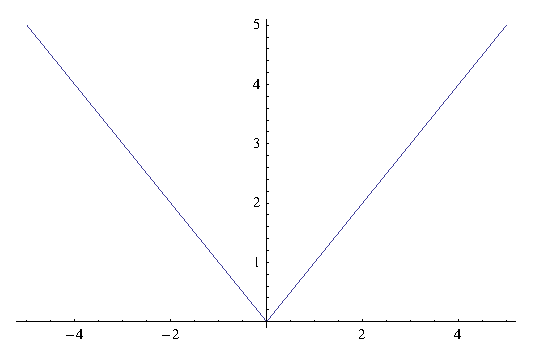
\includegraphics[width=0.5\textwidth]{sl1.eps}
\caption{Grafik funnkcije $f(x) = |x|$}
\end{center}
%Referenca na \cite{lit1}
\end{figure}

\par Zatim nacrtajmo sada grafik funkcije $|x-3|$, dobijamo kada pomerimo grafik udesno za 3 mesta po x-osi.
\newpage
\begin{figure}[h!]
\begin{center}
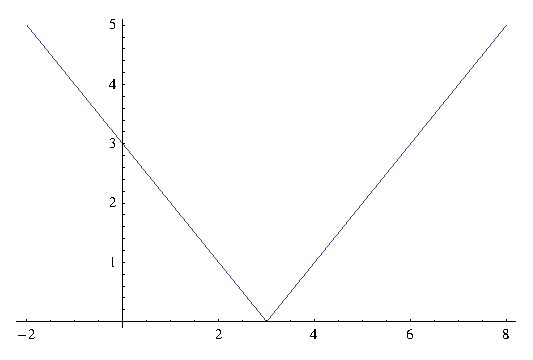
\includegraphics[width=0.5\textwidth]{sl2.eps}
\caption{Grafik funnkcije $f(x) = |x-3|$}
\end{center}
\end{figure}

\par Zatim nacrtajmo sada grafik funkcije $|x-3 | - 1$, dobijamo kada pomerimo grafik nadole za 1 mesto po y-osi.
\begin{figure}[h!]
\begin{center}
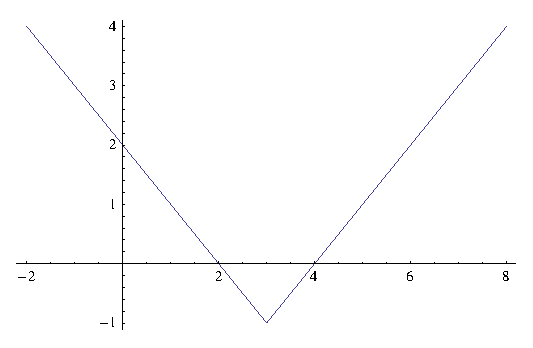
\includegraphics[width=0.5\textwidth]{sl3.eps}
\caption{Grafik funnkcije $f(x) = |x-3| -1$}
\end{center}
\end{figure}

\par Zatim nacrtajmo apsolutnu vrednost gornje funkcije to jest nacrtajmo $||x-3 | - 1|$, to se radi tako \v{s}to se sve ono \v{s}to je ispod x-ose simetri\v{c}no preslika iznad nje.
\begin{figure}[h!]
\begin{center}
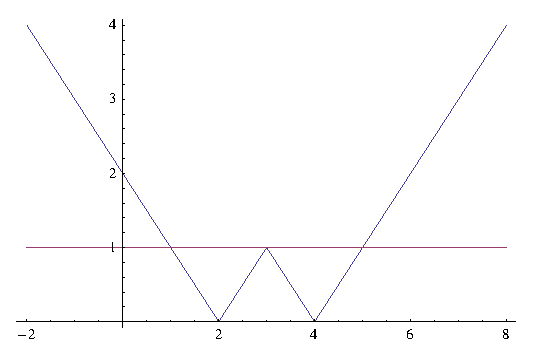
\includegraphics[width=0.5\textwidth]{sl4.eps}
\caption{Grafik funnkcije $f(x) =| |x-3| -1|$}
\end{center}
\end{figure}

\par Sa slike ve\'{c} uo\v{c}avamo da je re\v{s}enje prava $y = 1$, jer jedino ona se\v{c}e grafik u ta\v{c}no 3 ta\v{c}ke. To jest re\v{s}enje parametra $a$ je 1. \textbf{Odgovor je pod C.}

\item Krenemo od $f(x) = \frac{ax +b}{cx+d} $ i zamenjujemo redom vrednosti $x$, i gledamo \v{s}ta nam to re\'{c}i o funkciji $f$.
\par $f(0) = 1 \Longrightarrow f(0) = \frac{a \cdot 0 + b}{c \cdot 0 + d} = \frac{b}{d} = 1  \Longrightarrow  b = d$. Te znamo da je funckija $f(x)$ oblika $\frac{ax+b}{cx+b}$. Zatim,
\par $f(1) = 0 \Longrightarrow f(1) = \frac{a \cdot 1 + b}{c \cdot 1 + b} = \frac{a+b}{c+b} = 0  \Longrightarrow  a+b = 0$ to jest $a = -b$. Te dobijamo da je funckija $f(x)$ oblika $\frac{-bx+b}{cx+b}$. A iz
\par $f(2) = 3 \Longrightarrow f(2) = \frac{-b \cdot 2 + b}{c \cdot 2 + b} = \frac{-b}{2c+b} = 3  \Longrightarrow  -b = 3 \cdot (2c+b)$, naravno za $2c+b \neq 0$, dobijamo da je $-b = 6c +3b \Longrightarrow c = - \frac{2}{3} b$.
\par Iz svegda ovoga zaklju\v{c}ujemo daje fukcija $f(x)$ oblika $\frac{-bx + b}{- \frac{2}{3} b x + b} $, kada podelimo brojioc i imenioc sa $b$ dobijamo da je $f(x) =\frac{-x + 1}{- \frac{2}{3} x + 1} =\frac{1-x}{1- \frac{2}{3} x }  $.
\par Odatle mozemo da izra\v{c}unamo $f(3) =\frac{1-3}{1- \frac{2}{3} \cdot 3 } = \frac{-2}{1-2} = 2 $. \textbf{Odgovor je pod D.}


%12
\item Pogledajmo prvo sistem:
\begin{center}
\par $(x^{2} - 1)(2x -3y + 4z) = 0$
\par $4x + 5y +8z = -2$
\par $3x + y + 6z = 44$
\end{center}

\par Li\v{c}i na sitem 3 jedna\v{c}ina sa 3 nepoznate, samo \v{s}to nam smeta $(x^{2} - 1)$  iz prve jedna\v{c}ine. Pa hajmo da se re\v{s}imo toga. Kada je $x^{2} - 1 = 0$ to jest kada je $x^{2} =1$, o\v{c}igledmo je za $x = \pm 1$.
\par Razmatra\'{c}emo tri slu\v{c}aja kada je $x = 1$, $x+ -1$ i kada je $x \neq \pm 1$.
\begin{enumerate}[1)]

\item Kada je $x = 1$ dobijamo sistem:
\begin{center}
\par $4 + 5y +8z = -2$
\par $3 + y + 6z = 44$
\end{center}
\begin{center}
\par $5y +8z = -6$
\par $y + 6z = 41$
\end{center}
\par Izrazimo sada $y$:
\begin{center}
\par $5y +8z = -6$
\par $y = 41 - 6z$
\end{center}
\par Zamenimo $y$ u gornju jedna\v{c}inu:
\begin{center}
\par $5 \cdot (41 - 6z) +8z = -6$
\par $y = 41 - 6z$
\end{center}
\begin{center}
\par $205 -30z +8z = -6$
\par $y = 41 - 6z$
\end{center}
\begin{center}
\par $-22z = -211$
\par $y = 41 - 6z$
\end{center}
\par Izra\v{c}unamo sada $z$:
\begin{center}
\par $z = \frac{211}{22}$
\par $y = 41 - 6z$
\end{center}
\par Zamenimo vrednos $z$ u donji izraz da bismo dobili $y$:
\begin{center}
\par $z = \frac{211}{22}$
\par $y = 41 - 6 \cdot \frac{211}{22} = - \frac{182}{11}  $
\end{center}
\par Te je re\v{s}enje sistema jedinstveno i glasi $(1,-\frac{182}{11}, \frac{211}{22})$.

\item Kada je $x = -1$ dobijamo sistem:
\begin{center}
\par $-4 + 5y +8z = -2$
\par $-3 + y + 6z = 44$
\end{center}
\begin{center}
\par $5y +8z = 2$
\par $y + 6z = 47$
\end{center}
\par Izrazimo sada y:
\begin{center}
\par $5y +8z = 2$
\par $y = 47 - 6z$
\end{center}
\par Zamenimo $y$ u gornju jedna\v{c}inu:
\begin{center}
\par $5 \cdot (47 - 6z) +8z = 2$
\par $y = 47 - 6z$
\end{center}
\begin{center}
\par $235-30z +8z = 2$
\par $y = 47 - 6z$
\end{center}
\begin{center}
\par $-22z=-233$
\par $y = 47 - 6z$
\end{center}
\begin{center}
\par $z = \frac{233}{22}$
\par $y = 47 - 6z$
\end{center}
\par Zamenimo vrednos $z$ u donji izraz da bismo dobili $y$:
\begin{center}
\par $z = \frac{233}{22}$
\par $y = 47 - 6 \cdot \frac{233}{22} = - \frac{182}{11}$
\end{center}
\par Te je re\v{s}enje sistema jedinstveno i glasi $(1,-\frac{182}{11}, \frac{211}{22})$.

\item Po\v{s}to je $x \neq \pm 1$, onda prvu jedna\v{c}inu mo\v{z}emo podeliti sa $(x^2 - 1)$, i re\v{s}avamo sistem:
\begin{center}
\par $2x -3y + 4z = 0$
\par $4x + 5y +8z = -2$
\par $3x + y + 6z = 44$
\end{center}
\par Ovaj sistem je 3x3 pa se malo te\v{z}e re\v{s}ava. Mo\v{z}emo uo\v{c}iti linearnu zavisnost jedna\v{c}ina i lako je pokazati. Pomno\v{z}imo prvu jedna\v{z}inu sa -2 i dodamo je drugoj, i sa $-\frac{3}{2}$ i dodamo je tre\'{c}oj. Tim dobijamo:
\begin{center}
\par $2x -3y + 4z = 0$
\par $11y = -2 \Longrightarrow y = -\frac{11}{2}$
\par $\frac{11}{2}y = 44 \Longrightarrow y = 8$
\end{center}
\par Ovime smo dobili kontradikciju, to jest da ovaj sistem nema re\v{s}enje.
\end{enumerate}
\par Zaklju\v{c}ak je da polazni sistem ima samo dva re\v{s}enja.\textbf{Odgovor je pod C.} 

\textbf{Ubaciti laksi nacin resavanja ovog zadataka, bez bukvalnog racunanja}

\item Pogledajmo polazni sistem:
\begin{center}
\par $7 \cdot 3^{x} - 5 \cdot 2^{y} = 23$
\par $2 \cdot 3^{x} + 3 \cdot 2^{y} = 42$
\end{center}
\par Uvodimo smenu $a = 3^x, b = 2^y$, tada nam sistem izgleda:
\begin{center}
\par $7 a - 5b = 23$
\par $2 a + 3 b = 42$
\end{center}
\par Ovo je sistem linearnih jedna\v{c}ina sa dve nepoznate koji se jako lako re\v{s}i, i njegova re\v{s}enja su:
\begin{center}
\par $a = 9$
\par $b = 8$
\end{center}
\par Pa je re\v{s}enje polaznog sistema:
\begin{center}
\par $3^x = a = 9\Longrightarrow x = 2$
\par $2^y = b = 8 \Longrightarrow y = 3$
\end{center}
\par Tra\v{z}eni izraz $x+y = 5$. \textbf{Odgovor je pod E.}

\item Da bismo ovo re\v{s}ili treba da znamo svojstva logaritma. Ona koja su nam ovde potrebna su: $\log_{a^n} b = \frac{1}{n} \log_a b$, $\log_a b^n = n \log_a b$, $\log_a a = 1$ i  $\log_a b + \log_a c = \log_a bc$.
\begin{center}
\par $ \log_{36} x^{2} + \log_6 (x + 5) -1 = 0$
\par $ \log_{6^2} x^{2} + \log_6 (x + 5) = 1$
\par $ \frac{1}{2} \log_6 x^{2} + \log_6 (x + 5) = 1$
\par $ \frac{1}{2} \cdot 2 \cdot \log_6 |x| + \log_6 (x + 5) = 1$
\end{center}
\par Ovde mora $|x|$ jer nije nazna\v{c}eno koji je domen u pitanju.
\begin{center}
\par $ \log_6 |x| + \log_6 (x + 5) = 1$
\par $ \log_6 |x|(x + 5) = 1$
\par $ \log_6 |x|(x + 5) = \log_6 6$
\par $|x|(x + 5) = 1$
\end{center}
\par Razmatramo sada dva slu\v{c}aja:
\begin{enumerate}[1)]
\item Kada je $x > 0$: $x(x+5) = 6 \Longrightarrow x^2 + 5x -6 = 0 \Longrightarrow (x+6)(x-1)=0$. Re\v{s}enje za ovaj slu\v{c}aj je $x = 1$.
 
\item Kada je $-5 < x- < 0$:  $-x(x+5) = 6 \Longrightarrow -x^2 - 5x -6 = 0 \Longrightarrow -(x+3)(x+2)=0$. Re\v{s}enja za ovaj slu\v{c}aj je $x = -2$ i  $x = -3$.
\par Napomena: Kada je logaritam u pitanju, ono sto je pod njim ne sme biti 0, stoga se samo razmatra kada je $x$ manje od 0. Tako\dj{}e gore imam $log_6 (x+5)$ odakle uzimamo drugo ograni\v{c}enje a to je da $x+5>0$ to jest $ x > -5$.
\end{enumerate}
\par Proizvod re\v{s}enja je $1 \cdot 2 \cdot 3 = 6$. \textbf{Odgovor je pod E.} 


\item Posmatrajmo prvo interval od $[0,\pi]$. Na intervalu $[0, \frac{\pi}{4}) \sin x < \cos x$, a na intervalu $\frac{3\pi}{4}, \pi] \sin x < |\cos x|$, dok na ostalim delovim u okviru $[o,\pi]$ uslov nije ispunjen.
\par Kada imamo to uo\v{c}eno razmotrimo sada neke aproksimacije koje \'{c}e nam pomo\'{c}i za dalji razmatranje: $\frac{\pi}{4} = 0.735, \frac{3\pi}{4} = 2.305, \pi = 3.14, 2\pi = 6.28, 2\pi + \frac{pi}{4} =\frac{9\pi}{4} = 7.015,2\pi + \frac{3pi}{4} =\frac{11\pi}{4} = 8,585, 3\pi = 9.42$.
\begin{itemize}
\item $x in [0,\frac{\pi}{4})\rightarrow $ re\v{s}enje je 0.
\item $x in (\frac{3\pi}{4}, \pi] \rightarrow $ re\v{s}enje je 3.
\item $x in [\pi, 2\pi) \rightarrow $ re\v{s}enja su 4,5,6.
\item $x in [2\pi, \frac{9\pi}{4}) \rightarrow $ re\v{s}enje je 7.
\item $x in (\frac{11\pi}{4}, 3\pi] \rightarrow $ re\v{s}enja nema, jer je ovo disjunktno sa $[0,8]$.
\end{itemize}
\par Broj re\v{s}enja je 6.\textbf{Odgovor je pod C.} 


%16,17,18
\item 16 MITA
\item 17 MITA
\item 18 I MITA

\item Pogledajmo jedna\v{c}ine pravih $2x + y - 3 = 0$, $2x +y -8 = 0$. Zapi\v{s}imo ih malo druga\v{c}ije $y = -2x +3$, $y=  2x + 8$. Vidimo da su koeficijenti pravca jednaki te da su prave paralelne. Da bismo dobili ivicu kvadrata dovoljno je naci rastpojanje ime\dj{}u pravih. To \'{c}emo na\'{c}i tako \v{s}to \'{c}emo uzeti neku ta\v{c}ku sa jedna prave, i na\'{c}i njeno rastojanje od druge prave.
\par Uze\'{c}u ta\v{c}ku sa prve prave, i neka to bude ta\v{c}ka u kojoj $x$ uzima vrednost 0. To \'{c}e biti ta\v{c}ka gde je $y = -2 \cdot 0 +3 = 3$, to jest ta\v{c}ka $(0,3)$. Koriste\'{c}i formulu za nala\v{z}enje odstojanaj ta\v{c}ke od prave nalazimo ivicu kvadrata $a$: (Neka je prava $q$ zadata jedna\v{c}inom $ 2x+y-8 = 0$)
\par $d((0,3), q) = \frac{|2 \cdot 0 + 1 \cdot 3 -8|}{\sqrt{2^2 + 1^2}} = \frac{|-5|}{\sqrt{5}} = \sqrt{5}$
\par Dobijemo da je $a = \sqrt{5}$ to jest povr\v{s}ina kvadrata je 5. \textbf{Odgovor je pod B.} 


\item Kako imamo $a,b,\sin{\alpha} $ mo\v{z}emo koriste\'{c}i sinusnu teorenu da na\dj{}emo i $\sin{\beta}$:
\par $ \frac{a}{\sin{\alpha}}= \frac{b}{\sin{\beta}}  \Longrightarrow \frac{60}{\frac{12}{13}}= \frac{52}{\sin{\beta}} \Longrightarrow \sin{\beta} = \frac{4}{5} $
\par Kako imamo sinuse uglove, mo\v{z}emo lako na\'{c}i konsinuse iz relacije $\sin^2  x  +\cos^2  x  = 1$, a kako su to uglovi trougla znamo da \'{c}e vrednosti biti pozitivne. Sa lako\'{c}om nalazimo $\cos{\alpha} = \frac{5}{13}, \cos{\beta} = \frac{3}{5} $.
\par Po\v{s}to je $\gamma = \pi - \alpha - \beta$ imamo: 
\par $\sin{\gamma} = \sin(\pi - \alpha - \beta)= \sin( \alpha + \beta) = \sin{\alpha}\cos{\beta} + \sin{\beta} \cos{\alpha} = \frac{12}{13}\cdot \frac{3}{5} + \frac{5}{13}  \cdot \frac{4}{5} = \frac{36+20}{65} = \frac{56}{65} $. \textbf{Odgovor je pod A.}





\end{enumerate}



%\section{Kratak istorijski pregled}
%\par Kao što smo već istakli, postojanje familija asteroida prvi je primetio japanski astronom Hirajama još daleke 1918. godine. Trudićemo se da ovde damo što je moguće potpuniji pregled svega što se tokom proteklog stoleća dešavalo na ovom polju.

%\begin{figure}[!h]
%\begin{center}
%\includegraphics[width=0.4\textwidth]{slika16.jpg}
%\caption{Japanski astronom Kiotsugu Hirajama prvi je primetio postojanje familije asteroida}
%\end{center}
%\end{figure}
%\begin{itemize}
%\item familije asteroida postoje i mogu se pouzdano identifikovati
%\item familije su nastale sudarom dva asteroida.
%\item članovi familije ne predstavljaju dominantnu populaciju kod malih asteroida.
%\item u trenutku nastanka familije njeni članovi nisu izbačeni velikim brzinama.
%\item familije su značajno evoluirale u odnosu na post-sudarnu situaciju.
%\item inicijalno polje brzina teško da može biti rekonstruisano.
%\item starost familija se može odrediti.
%\item članovi familija su većinom re-akumulirani.
%\item asteroidi koji su predstavljali roditeljska tela familija nisu bili diferencirani.
%\end{itemize}

%Literatura
%\href{http://www.wikibooks.org}{Wikibooks home}
\begin{thebibliography}{9}
\bibitem{lit1} kkkk
\bibitem{lit2} kkkkk

\end{thebibliography}


\end{document}
